\section{Questions}


\begin{enumerate}
    \item The justification for performing two-dimensional analysis for a three dimensional object is the flux is only happening in the x, y direction and the length of the object in the z direction is small compared to the direction in the x and y. We also assume the Biot number in the z axis is  small.
    \item We defined the top and right boundary layers as having constant temperature therefore in the implementation we will set their temperature and not change their values. The boundary condition for the interior node is defined as the following:
    % Interior node
    \begin{equation}
    \begin{gathered}
        \rho { c }_{ p }\Delta x\Delta y\frac { { { { T }_{ ij } }^{ p+1 }-{ { T }_{ ij } }^{ p } } }{ \Delta t } =\left( k \right) \left( \Delta y \right) \left( \frac { { T }_{ i-1,j }-{ T }_{ ij } }{ \Delta x }  \right) +\left( k \right) \left( \Delta y \right) \left( \frac { { T }_{ i+1,j }-{ T }_{ ij } }{ \Delta x }  \right) \\
        %
        +\left( k \right) \left( \Delta x \right) \left( \frac { { T }_{ i,j-1 }-{ T }_{ ij } }{ \Delta y }  \right) +\left( k \right) \left( \Delta x \right) \left( \frac { { T }_{ i,j+1 }-{ T }_{ ij } }{ \Delta y }  \right) +\dot { q } \left( \Delta x \right) \left( \Delta y \right) 
    \end{gathered}
    \end{equation}
    % Bottom nodes of the grid
    The bottom boundary layer node which experiences a constant heat flux is written as the following:
    \begin{equation}
    \begin{gathered}
        \rho { c }_{ p }\Delta x\frac { \Delta y }{ 2 } \frac { { { { T }_{ ij } }^{ p+1 }-{ { T }_{ ij } }^{ p } } }{ \Delta t } ={ q }^{ " }\Delta x+\left( k \right) \left( \frac { \Delta y }{ 2 }  \right) \left( \frac { { T }_{ i-1,j }-{ T }_{ ij } }{ \Delta x }  \right) \\
        %
        +\left( k \right) \left( \frac { \Delta y }{ 2 }  \right) \left( \frac { { T }_{ i+1,j }-{ T }_{ ij } }{ \Delta x }  \right) +\left( k \right) \left( \Delta x \right) \left( \frac { { T }_{ i,j+1 }-{ T }_{ ij } }{ \Delta y }  \right)+\dot { q } \left( \Delta x \right) \left( \frac { \Delta y }{ 2 }  \right) 
    \end{gathered}
    \end{equation}
    %Left Node of the grid
    The left boundary layer node which experiences a constant heat flux from the left is written as the following:
    \begin{equation}
    \begin{gathered}
        \rho { c }_{ p }\Delta y\frac { \Delta x }{ 2 } \frac { { { { T }_{ ij } }^{ p+1 }-{ { T }_{ ij } }^{ p } } }{ \Delta t } ={ q }^{ " }\Delta y+\left( k \right) \left( \Delta y \right) \left( \frac { { T }_{ i+1,j }-{ T }_{ ij } }{ \Delta x }  \right) \\
        %
        +\left( k \right) \left( \frac { \Delta x }{ 2 }  \right) \left( \frac { { T }_{ i,j+1 }-{ T }_{ ij } }{ \Delta y }  \right) +\left( k \right) \left( \frac { \Delta x }{ 2 }  \right) \left( \frac { { T }_{ i,j-1 }-{ T }_{ ij } }{ \Delta y }  \right) +\dot { q } \left( \frac { \Delta x }{ 2 }  \right) \left( \Delta y \right) 
    \end{gathered}
    \end{equation}
    %Corner Node
    The corner boundary layer which has heat flux coming from both the left and the bottom equation is defined as the following:
    \begin{equation}
    \begin{gathered}
        \rho { c }_{ p }\frac { \Delta y }{ 2 } \frac { \Delta x }{ 2 } \frac { { { { T }_{ ij } }^{ p+1 }-{ { T }_{ ij } }^{ p } } }{ \Delta t } ={ q }"\frac { \Delta x }{ 2 } +q"\frac { \Delta y }{ 2 } \\
        %
        +\left( k \right) \left( \frac { \Delta y }{ 2 }  \right) \left( \frac { { T }_{ i+1,j }-{ T }_{ ij } }{ \Delta x }  \right) +\left( k \right) \left( \frac { \Delta x }{ 2 }  \right) \left( \frac { { T }_{ i,j+1 }-{ T }_{ ij } }{ \Delta y }  \right) +\dot { q } \left( \frac { \Delta x }{ 2 }  \right) \left( \frac { \Delta y }{ 2 }  \right) 
    \end{gathered}
    \end{equation}
    %
    %
    \item We can rearrange the internal node into the following forms:
    % \begin{equation}
    %     { { T }_{ ij } }^{ p+1 }=\frac { \Delta t }{ \rho { c }_{ p }\Delta x\Delta y } \left( \frac { k\Delta y }{ \Delta x } \left( { T }_{ i-1,j }-{ T }_{ ij } \right) +\frac { k\Delta y }{ \Delta x } \left( { T }_{ i+1,j }-{ T }_{ ij } \right) +\frac { k\Delta x }{ \Delta y } \left( { T }_{ i,j-1 }-{ T }_{ ij } \right) +\frac { k\Delta x }{ \Delta y } \left( { T }_{ i,j+1 }-{ T }_{ ij } \right) +\dot { q } \left( \Delta x \right) \left( \Delta y \right)  \right) +{ { T }_{ ij } }^{ p }
    % \end{equation}
    \begin{equation}
        { { T }_{ ij } }^{ p+1 }=\frac { -2\Delta t }{ \rho { c }_{ p }\Delta x\Delta y } \left( \frac { k\Delta y }{ \Delta x } +\frac { k\Delta y }{ \Delta y }  \right) { { T }_{ ij } }^{ p }+{ { T }_{ ij } }^{ p }+\cdots
        %
        %{ { T }_{ ij } }^{ p+1 }=\frac { -2\Delta t }{ \rho { c }_{ p }\Delta x\Delta y } \left( \frac { k\Delta y }{ \Delta x } +\frac { k\Delta y }{ \Delta y }  \right) { { T }_{ ij } }^{ p }+{ { T }_{ ij } }^{ p }+\frac { \Delta t }{ \rho { c }_{ p }\Delta x\Delta y } \left( \frac { k\Delta y }{ \Delta x } \left( { T }_{ i-1,j } \right) +\frac { k\Delta y }{ \Delta x } \left( { T }_{ i+1,j } \right) +\frac { k\Delta x }{ \Delta y } \left( { T }_{ i,j-1 } \right) +\frac { k\Delta x }{ \Delta y } \left( { T }_{ i,j+1 } \right) +\dot { q } \left( \Delta x \right) \left( \Delta y \right)  \right)
    \end{equation}
    \begin{equation}
        { { T }_{ ij } }^{ p+1 }=\left( 1+\frac { -2k\Delta t }{ { \rho { c }_{ p }\Delta x }^{ 2 } } +\frac { -2k\Delta t }{ { \rho { c }_{ p }\Delta y }^{ 2 } }  \right) { { T }_{ ij } }^{ p }+\cdots 
        %{ { T }_{ ij } }^{ p+1 }=\left( 1+\frac { -2k\Delta t }{ { \rho { c }_{ p }\Delta x }^{ 2 } } +\frac { -2k\Delta t }{ { \rho { c }_{ p }\Delta y }^{ 2 } }  \right) { { T }_{ ij } }^{ p }+\frac { \Delta t }{ \rho { c }_{ p }\Delta x\Delta y } \left( \frac { k\Delta y }{ \Delta x } \left( { T }_{ i-1,j } \right) +\frac { k\Delta y }{ \Delta x } \left( { T }_{ i+1,j } \right) +\frac { k\Delta x }{ \Delta y } \left( { T }_{ i,j-1 } \right) +\frac { k\Delta x }{ \Delta y } \left( { T }_{ i,j+1 } \right) +\dot { q } \left( \Delta x \right) \left( \Delta y \right)  \right)
    \end{equation}
    Thus if the grid spacing is equal in both equal, we can combine the terms in front of the ${ { T }_{ ij } }^{ p }$ and look at the stability. We can see that the $F_{0}$ must be less then 0.25 and inversely the time must not make the value of $F_{0}$ increase pass 0.25.
    \begin{equation}
        \left( 1-\frac { 4k\Delta t }{ { \rho { c }_{ p }\Delta x }^{ 2 } }  \right) \geq 0
    \end{equation}
    \begin{equation}
        \left( 1-4{ F }_{ 0 } \right) \geq 0\ \text{thus}\ { F }_{ 0 }\le 0.25
    \end{equation}
    \item The material of choice for this numerical analysis of the plate was Aluminum Alloy 2024-T6 (values used in the experiment can be found in Table A-1 in the book). For 31 nodes in both the X and Y direction with a temperature distribution after 360 seconds and a ${\dot{q}}$=0 the results can be seen below in Figure \ref{fig_q4_1}.
    %
    \begin{figure}[H]
        \centering
        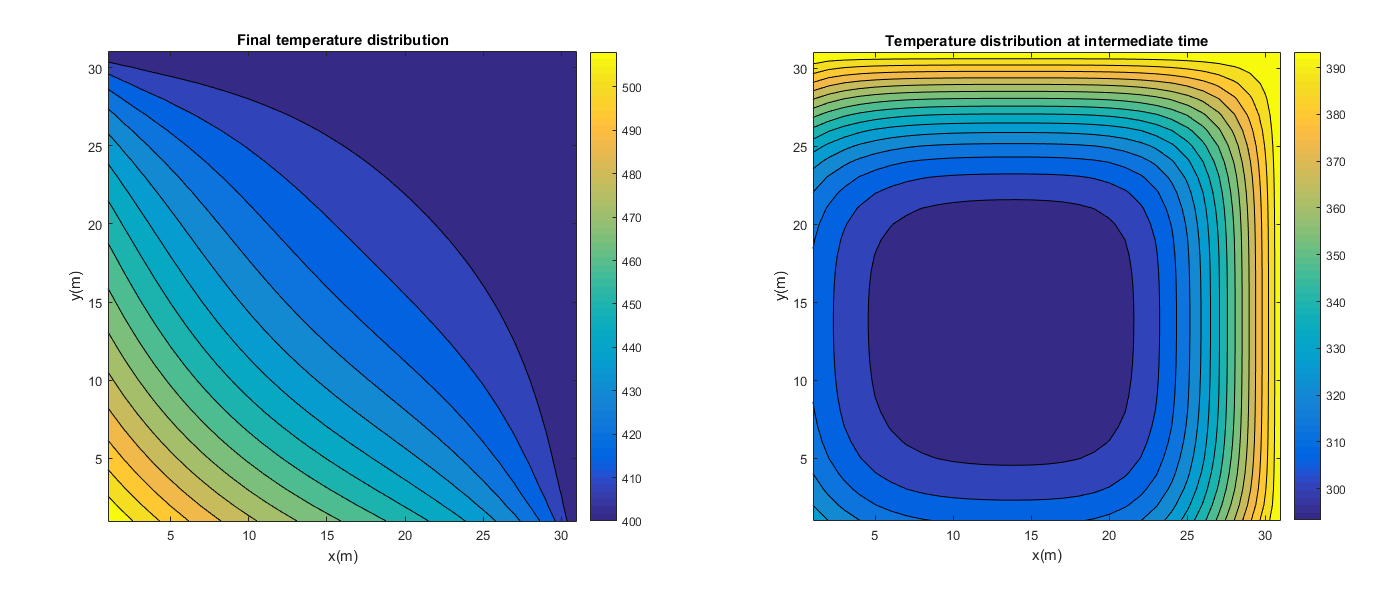
\includegraphics[width=5in]{pictures/time_360_31_0.png}
        \caption{}
        \label{fig_q4_1}
    \end{figure}
    %
    The temperature distribution after 2000 seconds with a ${\dot{q}}$=1 W/${ cm }^{ 3 }$ as seen in Figure \ref{fig_q4_3}.
    %
    \begin{figure}[H]
        \centering
        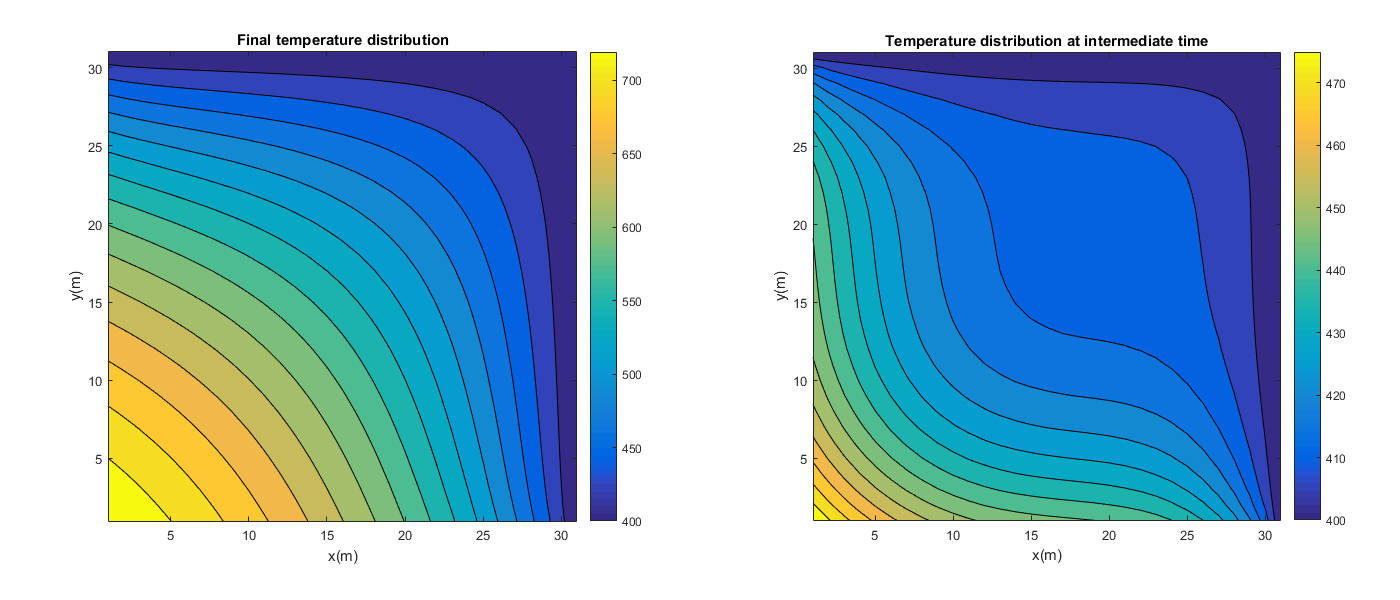
\includegraphics[width=5in]{pictures/time_2000_31_1.png}
        \caption{}
        \label{fig_q4_3}
    \end{figure}
    %
    The summary of the results, including runs with higher node counts, can be seen in the table below. Based on these results, it can be found that the more nodes used to analysis the plate, the lower the percent error since there are more data points to extrapolate from. Also, a longer period of time allowed the heat transfer to travel farther into the plate until steady state was reached.
    %
    \begin{center}
    \begin{tabular}{r r r r r}
        \label{table_q4_1}
        Nodes (\#) & Time (s) & Heat Rate (Watts) & Generated (W) & Error (\%) \\ \hline
        31         & 360      & -25500.0       & 0             & 100        \\
        61         & 360      & -26100.0       & 0             & 100        \\
        31         & 2000     & 91000.0        & 90000         & 1.0930     \\
        61         & 2000     & 90500.0        & 90000         & 0.5912     \\
    \end{tabular}
    \end{center}
    %
    \item The total energy leaving the plate is calculated by looking at the second and third row/column of nodes at the edges. The difference between these can be representative of what is the total heat is leaving the unit. Please see the table below for the summarized results.
    %
    \begin{center}
    \begin{tabular}{r r r r r}
        \label{table_q5_1}
        Nodes (\#) & Time (s) & Heat Rate (Watts) & Generated (W) & Error (\%) \\ \hline
        31         & SS       & 1320.0         & 0             & 100        \\
        61         & SS       & 670.39         & 0             & 100        \\
        31         & SS       & 91052.0        & 90000         & 1.1553     \\
        61         & SS       & 90593.0        & 90000         & 0.6542     \\
    \end{tabular}
    \end{center}
    %
    \item Figure \ref{fig_q6_1} shows the steady state temperature distribution after 8258.1 minutes of real world time. This is with no heat generation and with a 31 by 31 node grid.
    %
    \begin{figure}[H]
        \centering
        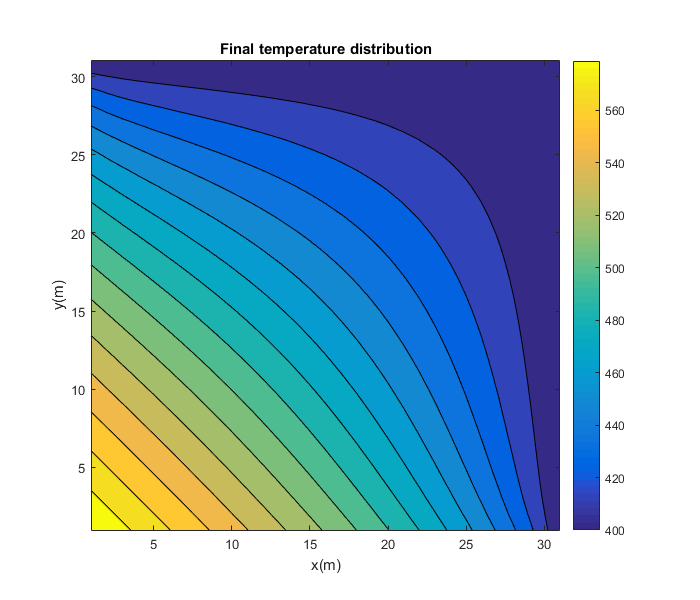
\includegraphics[width=3in]{pictures/time_SS_31_0.png}
        \caption{}
        \label{fig_q6_1}
    \end{figure}
    %
    \item In Figure \ref{fig_q7_1}, the maximum error is 7.49\%. The steady state temperature distribution across the diagonal of the plate for the numerical solution begins linear and turns into an exponential curve. The analytical solution, which uses the equation from lecture 11 slide 7, was found to be above the numerical solution later converging to the numerical solution. It is important to note that the error function matches the physical properties of the experiment. The error is high where there is flux, and it goes to zero as it approaches the constant temperature boundaries.   
    %
    \begin{figure}[H]
        \centering
        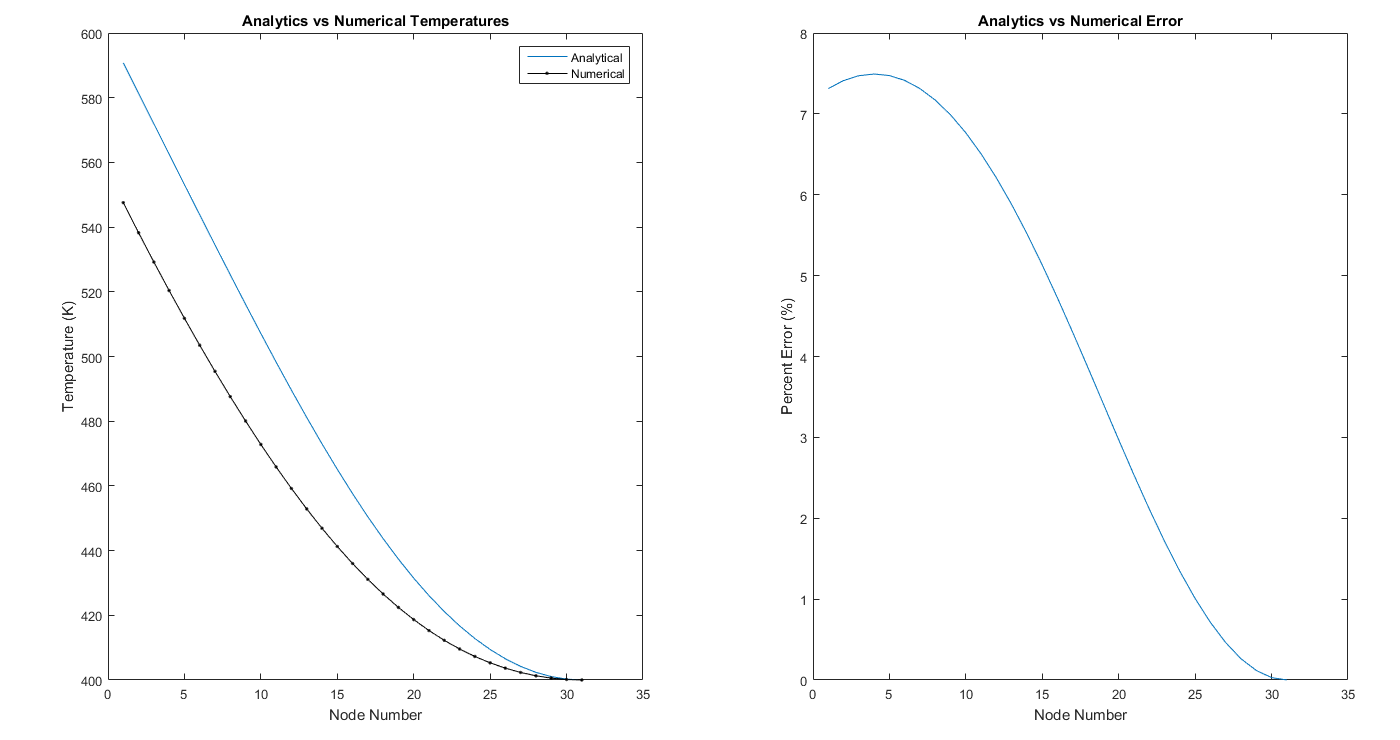
\includegraphics[width=6in]{pictures/diag_error.png}
        \caption{}
        \label{fig_q7_1}
    \end{figure}
    %
    \item To create a numerical instability, a $F_{0}$ number of 0.4 was selected. This corresponded to time steps of 0.5479 seconds. As seen below in Figure \ref{fig_q8_1} the simulation breaks down and has numerical issues (viewed graphically here as distortions/invalid values in the contour plot).
    %
    \begin{figure}[H]
        \centering
        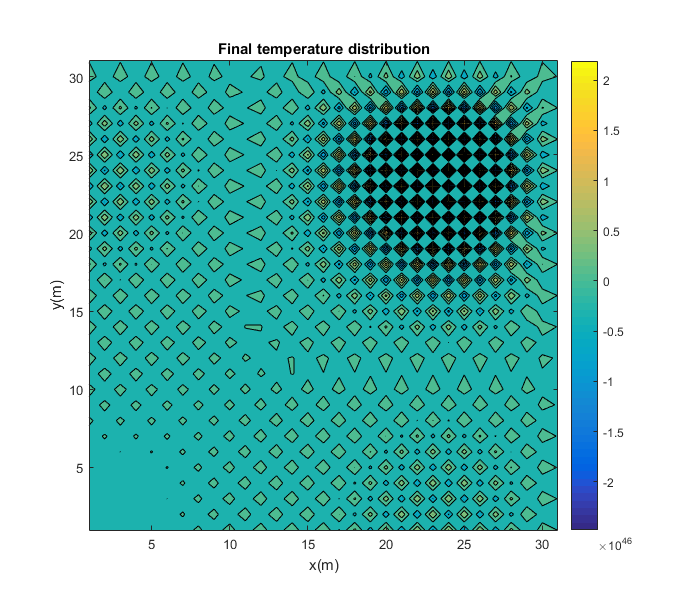
\includegraphics[width=3in]{pictures/instablity_example.png}
        \caption{}
        \label{fig_q8_1}
    \end{figure}
    
\end{enumerate}